\documentclass[11pt]{article}
%\author{Manish Prasad 18122012 EPH\\
%Supervisor: Prof. Rajdeep Chatterjee}
\usepackage{amsmath}
\usepackage{float}
\usepackage{graphicx}
\usepackage{subfig}
\numberwithin{equation}{section}
\usepackage{natbib}
\usepackage{hyperref}

\begin{document}
%\title{Applications of q-Statistics in Big Bang Nucleosynthesis}
%\maketitle


\begin{titlepage}
\begin{center}
 
 {\huge\bfseries Applications of q-Statistics in \\ Big Bang Nucleosynthesis\\}
 % ----------------------------------------------------------------
 \vspace{1.4cm}
 {A Project Report} \\
 {Submitted for the degree of} \\[1.1cm]
 {\Large\bfseries Bachelor of Technology}\\[5pt]
 {in}\\[8pt]
 {\Large\bfseries Engineering Physics}\\[5pt]
 \vspace{1.2cm}
 Submitted by:\\[5pt]
 {\Large\bfseries Manish Prasad}\\[8pt]
 Under the supervision of:\\[5pt]
 {\Large\bfseries \href{https://ph.iitr.ac.in/~PH/rcfphfph}{Dr. Rajdeep Chatterjee}}\\
\vspace{1.2cm} 
 \begin{figure}[H]
  \centering
  
\includegraphics[width=0.3\linewidth]{"./Figures/logo.jpg"}
\end{figure}
\href{https://ph.iitr.ac.in/}{\textbf{Department of Physics}}\\[5pt]
\href{https://iitr.ac.in/}{\textbf{Indian Institute of Technology, Roorkee}}\\[5pt]
{\textbf{Roorkee-247667 (India)}}\\[5pt]
{\textbf{April 2022}}
\end{center}
\end{titlepage}
\pagebreak

\begin{center}
  \Large\textbf{Candidate’s Declaration}
\end{center}
I hereby declare that the work, which is being presented in this report \\ entitled \textbf{“Applications of q-Statistics in Big Bang Nucleosynthesis”} and submitted in partial fulfilment of the requirements of the degree of Bachelor of Technology in Engineering Physics  as an authentic record of my own work carried out during the period of August 2021 to April 2022 under the supervision of \textbf{Dr. Rajdeep Chatterjee, Department of Physics, IIT Roorkee}. The matter contained in this report has not been submitted by me for the award of any other degree in the institute or any other Institute/University.

\vspace*{5em}\noindent

\begin{flushleft}

\includegraphics[width=0.3\linewidth]{"./Figures/sign.jpg"}\\
\textbf{Manish Prasad}\\
\textbf{B.Tech Engineering Physics}\\
\textbf{18122012}
\end{flushleft}
\pagebreak



\begin{center}
  \Large\textbf{Certificate}
\end{center}
This is to certify that the project entitled \textbf{“Applications of q-Statistics in Big Bang Nucleosynthesis”} is a bonafide work carried out by \\ Manish Prasad, B.Tech final year student IIT Roorkee, in the partial \\ fulfilment for the requirements of the award of the degree Bachelor of \\ Technology in Engineering Physics under my guidance.


\vspace*{10em}\noindent
\begin{flushleft}
\href{https://ph.iitr.ac.in/~PH/rcfphfph}{\textbf{Rajdeep Chatterjee}}\\
Professor\\
Department of Physics\\
Indian Institute of Technology Roorkee\\
\end{flushleft}
\pagebreak

\begin{center}
  \Large\textbf{Acknowledgement}
\end{center}
I would like to thank Dr. Rajdeep Chatterjee for his incredible support and motivation. He has encouraged me to explore the field of non-extensive statistics and nuclear astrophysics, even beyond the scope of this project. I have learnt a lot from him and I am happy that I got to work on a potential solution to the Lithium problem which is still an open ended problem. I am immensely grateful for his guidance. 



\pagebreak
\tableofcontents
\pagebreak

\section{Abstract}

This work describes the use of Tsallis non extensive statistics to calculate the abundances of light elements during big bang nucleosynthesis. The theory of Tsallis entropy, and it's impact on the Maxwell Boltzmann distribution was studied. Then, the new reaction rates were calculated using the non extensive statistics. The abundances of light nuclei were calculated using a BBN code and the impact of this q-parameter and the drawbacks of this model were discussed. 
\pagebreak


%\textbf{SBBN refers to BBN in the context of Einstein gravity, with a Friedmann-Lemaitre-Robertson-Walker cosmological background. It assumes the Standard Model of nuclear and particle physics, or in other words, the standard set of nuclear and particle interactions and nuclear and particle content. Read about SBBN in \cite{cyburt2016big}. Looks interesting.}




\section{q-Logarithm and q-Exponential Functions}

Consider the function $\dfrac{dy}{dx}=y^q$. The solution of this differential equation is:
$$y=[1+(1-q)x]^{1/(1-q)}$$
And the inverse is:
$$y=\frac{x^{1-q}-1}{1-q}$$
We can define these two solutions differently in the form of q-logarithm and q-exponential functions:
\begin{align}
	\ln_q x=\frac{x^{1-q}-1}{1-q}  \qquad (x>0;\; \ln_1 x=\ln x) \label{eq:lnq}\\
	e_{q}x=[1+(1-q)x]^{1/(1-q)}   \qquad (e_q^x=e^x)          \label{eq:expq}
\end{align}

We can see that as $q\to 1$, $ \lim_{q\to 1} ln_q x=ln x $ and $ \lim_{q\to 1} e_{q}^x=e^x $. We can also observe the following property:
\begin{equation}
	\ln_q (x_a x_b)=\ln_q x_a +\ln_q x_b + (1-q)\ln_q (x_a)\ln_q (x_b)
\end{equation}
More information about this can be found in Chapter 3 of \cite{tsallis2009introduction} and some important properties of the q-logarithm and q-exponential can be found in \cite{YAMANO2002486}. The graphs of the q-logarithm and q-exponential functions look like:

\begin{figure}[H]
	\centering
	\subfloat[q-Logarithm]{{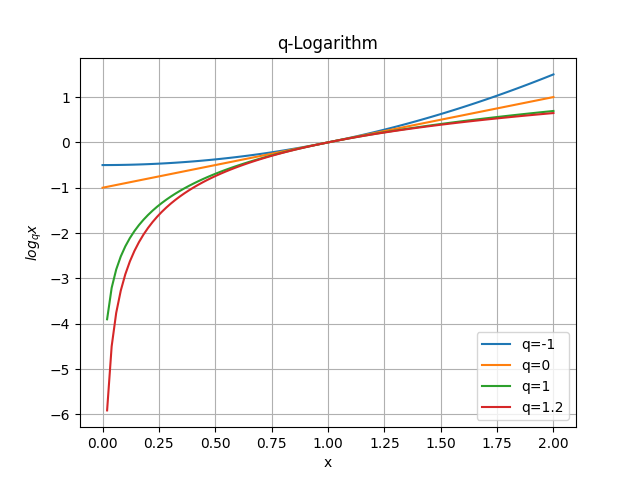
\includegraphics[width=.5\linewidth]{./Figures/q_log.png}}}
    \subfloat[q-Exponential]{{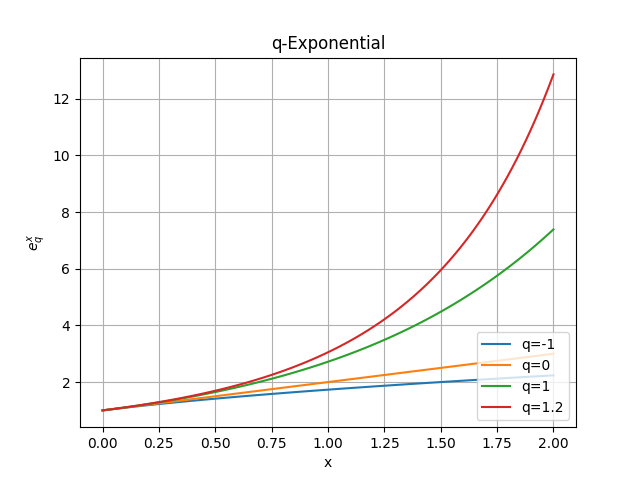
\includegraphics[width=.5\linewidth]{./Figures/q_exp.png}}}
	\caption{Graphs of q-Logarithm and q-Exponential plotted using Python}
	\label{q_log}
\end{figure}

\section{Tsallis Entropy}
\subsection{Boltzmann-Gibbs Entropy}
The Boltzmann–Gibbs (BG) entropy is given by (for a set of W discrete states):
\begin{equation}
	S_{BG}=-k\sum_{i=1}^{W} p_i \ln pi \qquad ;where\, \sum_{i=1}^{W} p_i=1 \label{SBG}
\end{equation}
Here k is a positive constant which is the Boltzmann constant $k_B$. For the  case of equal probabilities (i.e., $pi =1/W, \forall i$), Eq.\ref{SBG} becomes:
\begin{equation}
	S_{BG}=k\ln W \label{SBG p=1/w}
\end{equation}
We can observe the following property. If we compose two independent systems A and B (with numbers of states denoted by $W_A$ and $W_B$ respectively), such that the joint probabilities factorize, $p_{ij}^{A+B} = p_i^A p_j^B (\forall (i, j))$ and $W=W_A W_B$, then the entropy $S_BG$ is additive. That is:
\begin{equation}
	S_{BG}(A+B)=S_{BG}(A)+S_{BG}(B) \label{sum property}
\end{equation}
For a canonical system in thermal equilibrium at temperature T and its mean energy U, the BG statistical mechanics yields:
\begin{equation}
	\sum_{i=1}^{W}p_i E_i=U	\label{constraint piei}
\end{equation}
\begin{equation}
	p_i=\frac{e^{-\beta E_i}}{Z_{BG}} \label{eq:pi for SBG}
\end{equation}
where
\begin{align}
	\beta&=\frac{1}{kT}\\
	Z_{BG}&=\sum_{j=1}^{W} e^{-\beta E_j} \label{eq:Zq for SBG}
\end{align}
where $E_i$ denotes the energy spectrum and $Z_{BG}$ is the partition function of the system.\\ Equations \eqref{SBG} and \eqref{eq:pi for SBG} are the landmarks of BG statistical mechanics. and are successfully used in physics, mathematics, computer sciences, engineering, chemistry, etc. \\
But using the definitions in Chapter 1, Tsallis has generalized the BG statistics as a particular case of a more generalized distribution that has applications in many complex systems. For some systems, BG statistics becomes inefficiently applicable, and a generalization of the BG Statistical Mechanics proves to be helpful.

\subsection{Non-Additive Entropy}
Tsallis proposed the following generalization for \ref{SBG}
\begin{equation}
	S_q=k_b\ln_q W
\end{equation}
Using the definition in \eqref{eq:lnq}, we get:
\begin{equation}
	S_q=k_b\frac{1-\sum_{i=1}^{W}p_i^q}{q-1}
\end{equation}
where q is a parameter quantifying the degree of non-extensivity. We can see the variation of $S_q$ with W for different values of q in Figure \ref{fig:S_q with q}. Notice, for q=1, the figure corresponds to the BG Entropy.
\begin{figure}[H]
  \centering
  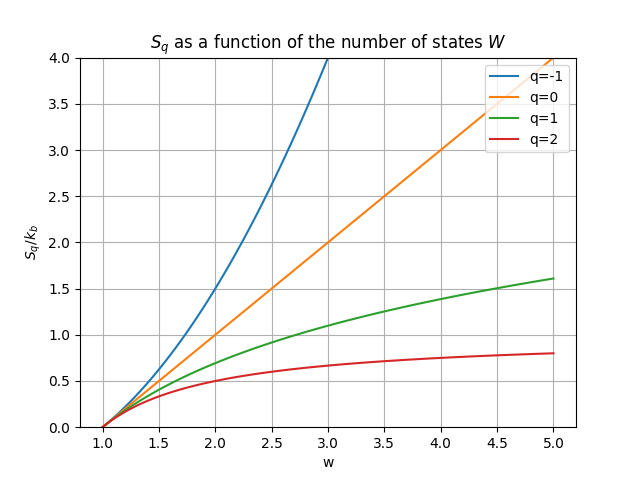
\includegraphics[width=0.9\linewidth]{"./Figures/S_q with w.png"}
  \caption{Equiprobability entropy Sq as a function of the number of states W, for some values of q}
  \label{fig:S_q with q}
\end{figure}
The property demonstrated in \eqref{sum property} now becomes:
\begin{equation}
	S_{q}(A+B)=S_{q}(A)+S_{q}(B)+ (1-q)S_{q}(A)S_{q}(B)
\end{equation}
For the non-extensive scenario, we need to extremize $S_q$ with the constraints $\sum_{j=1}^{W}p_i=1$ and $\sum_{j=1}^{W}p_i \varepsilon_i=U_q$. This can be done using \textit{Lagrange Multipliers}. This is solved in detail in \cite{tsallis1988possible} and we get the following results:
\begin{align}
	p_i&=\frac{[1-\beta(q-1)\varepsilon_i]^{1/q-1}}{Z_q}\nonumber\\
		&=\frac{[1+\beta(1-q)\varepsilon_i]^{-1/1-q}}{Z_q}\\ \label{eq:p_i for S_q}
		&=\frac{e_q^{-\beta\varepsilon_i}}{Z_q}\nonumber
\end{align}
where $\beta=1/k_b T$ and:
\begin{equation}
	Z_q=\sum_{i=1}^{W} [1-\beta(q-1)\varepsilon_i]^{1/q-1}=\sum_{i=1}^{W} e_q^{-\beta	} \label{eq:Zq for S_q}
\end{equation}
For $q\to 1$ we recover \ref{eq:pi for SBG} and \ref{eq:Zq for SBG}
\begin{figure}[H]
\centering
  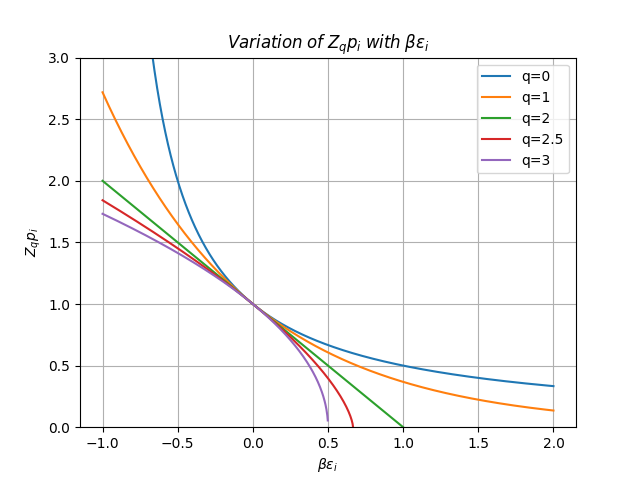
\includegraphics[width=0.9\linewidth]{"./Figures/p_i graph with z_q.png"}
  \caption{Variation of $Z_{q}p_{i}$ with $\beta\varepsilon_{i}$}
  \label{fig:p_i with z_q}
\end{figure}
From the Figure \ref{fig:p_i with z_q}, we can see that when $q>1$, we have a cutoff at:
\begin{equation}
	\beta\varepsilon_i=1/(q-1) \label{eq:cutoff}
\end{equation}
The equation \ref{eq:cutoff} will be useful during the discussion in Chapter \ref{section:5}
\section{Applications of Non-Extensive Statistics}
A brief introduction to Non extensive statistics is provided in \cite{asdfasdf}. Non-extensive statistics has a wide range of applications (Chapter 7 \cite{tsallis2009introduction})$\,$ in many fields like physics, chemistry, economics, computer sciences, biosciences, linguistics, etc. Following are three specific applications of q-statistics:
\begin{itemize}
    \item \textbf{Lithium Problem}: Big-bang nucleosynthesis (BBN) describes the production of the lightest nuclides such as elements like H, He, Li, and Be during the first seconds of cosmic time. But, the current theory overestimates the abundance of $^{7}Li$. And Tsallis statistics can be helpful in solving this. 
    \item \textbf{Cryptocurrency}: In \cite{STOSIC20181069}, a study of nonextensive behavior of daily price changes for cryptocurrencies like Bitcoin has been done, from 2013 until 2017. Their results strongly indicate that the cryptocurrency market represents a state whose physics can be described by nonextensive statistical mechanics.
    \item \textbf{Astrophysics: Temperature Fluctuations of the CMBR}: In the study of CMBR (Cosmic Microwave Background Radiation), q-Gaussians are used in astrophysics and they are called $\kappa$-distributions \cite{10.1007/978-94-010-3467-8_23}, and equations are identical to Equation \ref{eq:expq}.
\end{itemize}

\section{One Particle Maxwell Boltzmann Distribution and Tsallis Distribution}
\label{section:5}
The Maxwell Boltzmann distribution is given by:
\begin{equation}
	f_{MB}(v)=\left(\frac{m}{2\pi k_{B}T}\right)^{3/2}exp\left(-E/k_{B}T\right) \label{eq:MB 1 particle}
\end{equation} 
And the Tsallis distribution is given by:
\begin{equation}
	f_{q}(v)=B_{q}\left(\frac{m}{2\pi k_{B}T}\right)^{3/2}\left[1-(q-1)\frac{E}{k_{B}T}\right]^{1/q-1}
\end{equation}
Where $B_{q}$ is a normalization constant determined from the requirement $\int f_{q}(v_{i})dv_{i}=1$ and is given by:
\begin{equation}
	B_{q	}=(q-1)^{1/2}\left(\frac{3q-1}{2}\right)\left(\frac{1+q}{2}\right)\frac{\Gamma(\frac{1}{2}+\frac{1}{q-1})}{\Gamma(\frac{1}{q-1})}\left[\frac{m}{2\pi k_{B}T}\right]^{3/2}
\end{equation}
Derivation is given in \cite{Silva:1998iy} and furthur reading is provided in \cite{Kusakabe:2018dzx}.
We can further see that from the Equation \eqref{eq:cutoff}, there would be a cutoff for the Tsallis distribution. In the following figure \ref{fig:tsallis and maxwell}, for q=1.2 there will be a cutoff at:
\begin{equation}
	\frac{E}{k_b T}=\frac{1}{q-1}=\frac{1}{1.2-1}=5
\end{equation}
\begin{figure}[H]
  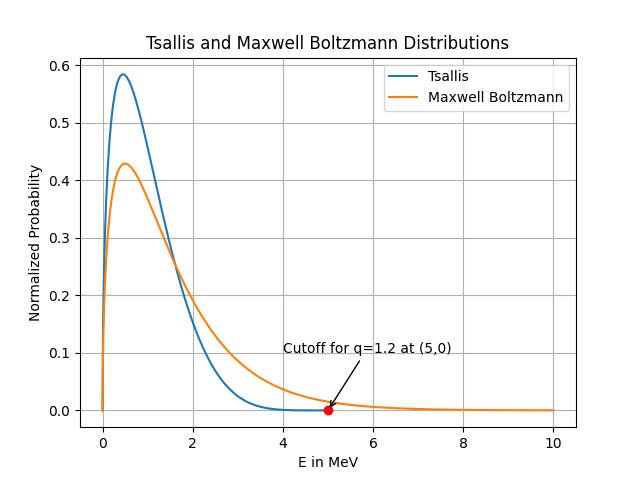
\includegraphics[width=\linewidth]{"./Figures/tsallis and mb.png"}
  \caption{Tsallis distribution (at q=1.2) and M-B distribution functions with $k_{B}T=1MeV$}
  \label{fig:tsallis and maxwell}
\end{figure}

\pagebreak
\section{Relative Velocity Distributions}
A detailed derivation of all the equations in this section is given in \citep{Kusakabe:2018dzx}. To derive the relative velocity distributions, the three conditions need to be satisfied are:
\begin{enumerate}
	\item Each nucleus is described by a non-Maxwell-Boltzmann velocity distribution
	\item Conservation of momentum
	\item Conservation of energy
\end{enumerate}
For a two particle system, let $m_{i}$ be the masses and $\boldsymbol{v_{i}}$ be the velocity vector of species i = 1 and 2. In the Center of Mass system, the total mass is M, the reduced mass is $\mu$ and \textbf{v} is the relative velocity:
\begin{align}
	M&=m_{1}+m_{2} \nonumber \\
	\mu&=\frac{m_{1}m_{2}}{m_{1}+m_{2}}\\
	\boldsymbol{v}&=\boldsymbol{v_{1}}-\boldsymbol{v_{2}} \nonumber
\end{align}
And the momentum and energy conservations lead to:
\begin{align}
	\boldsymbol{V}&=\frac{m_{1}\boldsymbol{v_{1}}+m_{2}\boldsymbol{v_{2}}}{m_{1}+m_{2}}\\
	m_{1}v_{1}^{2}&+m_{2}v_{2}^{2}=MV^{2}+\mu v^{2}
\end{align}
Hence, the distribution function of the relative velocity v is given by:
$$f^{rel}(\boldsymbol{v})= \int d\boldsymbol{V}\left [ f(\boldsymbol {v_{1}})f(\boldsymbol{v_{2}}) \right ]_{v}$$\
Where the term in brackets with the subscript \textbf{v} is estimated for a fixed v.
\subsection{Maxwell Boltzmann}
The CM distribution function of the relative velocity for the case of MB statistics has the same form as that of the individual particle distribution function \eqref{eq:MB 1 particle}:
\begin{equation}
	f^{rel}_{M}(\boldsymbol{v})=\frac{\mu^{3/2}}{(2\pi k_{B}T)^{3/2}}exp\left [ -\frac{\mu v^2}{2k_B T} \right ]
\end{equation}
\subsection{Tsallis Distribution}
\label{sec: tsallis dist}
The Tsallis distribution function of the relative velocity is given by:
$$f_{q}^{rel}(\boldsymbol{v})= \int d\boldsymbol{V}\left [ f_{q}(\boldsymbol {v_{1}})f_{q}(\boldsymbol{v_{2}}) \right ]_{v}$$
The ranges of V and v are calculated using \eqref{eq:cutoff}:
\begin{equation}
	m_{i}v_{i}^{2}\leq \frac{2k_{B}T}{q-1}
\end{equation}
Hence the ranges of V and v are:
\begin{align}
	0 &\leq V \leq \sqrt{\frac{2k_{B}T}{q-1}}\frac{\sqrt{m_{1}}-\sqrt{m_{2}}}{M}\\
	0&\leq v \leq v_{1,max} + v_{2,max}=\sqrt{\frac{2k_{B}T}{q-1}}\left( \frac{1}{\sqrt{m_{1}}} + \frac{1}{\sqrt{m_{2}}} \right)
\end{align}
Hence the distribution function becomes:
\begin{align}
	f_{q}^{rel}(v)&=2\pi \int_{-1}^{1} d\cos\theta\int_{0}^{V_{max}}V^{2}dV f_{q}(\boldsymbol{v_{1}})f_{q}(\boldsymbol{v_{2}}) \nonumber\\
	&=2\pi B_{q}^{2}\frac{(m_{1}m_{2})^{3/2}}{(2\pi k_{B}T)^{3/2}}\int_{-1}^{1} d\cos\theta\int_{0}^{V_{max}}V^{2}dV I_{q}(V,\cos\theta;m_{1},m_{2},T,v)
\end{align}
Where the function $I_{q}$ is given by:
\begin{equation}
	I_{q}(V,\cos\theta;m_{1},m_{2},T,v)=\left\{\begin{matrix}
=\left [ 1-(q-1)\frac{m_{1}v_{1}^{2}}{2k_{B}T} \right ]^{1/(q-1)} \left [ 1-(q-1)\frac{m_{2}v_{2}^{2}}{2k_{B}T} \right ]^{1/(q-1)} \\ v_{1}\leq v_{1,max}\; and\; v_{2}\leq v_{2,max} \\
=0 \qquad(otherwise)
\end{matrix}\right.
\end{equation}
And:
\begin{align}
	v_{1}^{2}&=V^{2}+2\frac{m_{2}}{M}Vv\cos\theta+\frac{m_{2}^{2}}{M^{2}}v^{2}\\
	v_{2}^{2}&=V^{2}-2\frac{m_{1}}{M}Vv\cos\theta+\frac{m_{1}^{2}}{M^{2}}v^{2}
\end{align}
The MB distribution $v_{th}^{3}f_{MB}^{rel}(v)$ depends only E/T	for a fixed q. The Tsallis distribution $v_{th}^{3}f_{q}^{rel}(v)$ depends on the nuclear masses as well as E/T for a fixed q. \emph{This is one of the important differences from MB statistics}
\begin{figure}[H]
  \includegraphics[width=\linewidth]{"./Figures/relative_distribution"}
  \caption{Normalized distributions for the center of mass energy E for q = 1.075. The dashed line is the one-particle Tsallis distribution. The dotted line corresponds to the MB distribution. The other line in between are for Tsallis statistics with (A1, A2) = (1, 1), (2, 2), (4, 3), (3, 2), (2, 1), (3, 1), and (7, 1) from top to bottom.  The graph is taken from \citep{Kusakabe:2018dzx}}
  \label{fig:relative_distribution}
\end{figure}


\section{q-Deformed Planck Distribution}
The q-Deformed Planck Distribution equation was derived in \citep{tsallis2009introduction}. The following equations are the normal Planck distribution and the q-deformed distribution.
\begin{align}
	N_{\gamma}(E_{\gamma})&=\frac{8\pi}{(hc)^{3}}\frac{E_{\gamma}^{2}}{e^{E_{\gamma}/k_{B}T}-1}dE_{\gamma}\\
	N_{q}(E_{\gamma})&=\frac{8\pi}{(hc)^{3}}\frac{E_{\gamma}^{2}}{e^{E_{\gamma}/k_{B}T}-1}(1-e^{-x})^{q-1}\Bigg\{1+(1-q)x\left[\frac{1+e^{-x}}{1-e^{-x}} - \frac{x}{2}\frac{1+3e^{-x}}{(1-e^{-x})^{2}}\right]\Bigg\}	dE_{\gamma}
\end{align}
\begin{figure}[H]
  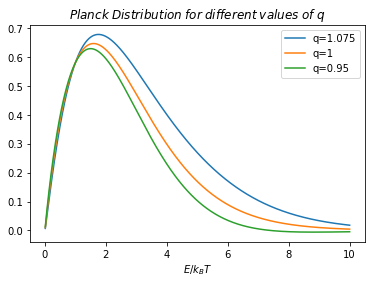
\includegraphics[width=\linewidth]{"./Figures/plank distribution.png"}
  \caption{q-Deformed Planck Distribution}
  \label{fig:q-plank}
\end{figure}

\section{Reaction Rates}
\subsection{Charged particle reaction rate}
For a charged particle reaction: $1+2\rightarrow3+4$, the reaction rate is given by:
$$r_{12}=N_{1}N_{2}\left< \sigma(v) v\right>$$
Where v is relative velocity of the particles 1 and 2, $N_{1}$ and $N_{2}$ are the number of particles of 1 and 2 per unit volume, $\sigma$ is the cross section, and $\left< \sigma v\right>$ is the average reaction rate per particle pair.
Since the particles will have a velocity distribution, in order to calculate $\left< \sigma v\right>$, we have to
integrate it over a velocity distribution.
$$\left< \sigma v\right>=\int f^{rel}(\boldsymbol{v})v\sigma(v)dv$$
The relation between $\sigma(E)$ and $S(E)$is:
\begin{equation}
	\sigma(E)=\frac{1}{E}S(E)e^{-2\pi\eta}
\end{equation}
Where $e^{-2\pi\eta}$ is the Gamow factor which gives the tunneling probability, and $\eta$ is Sommerfeld parameter.
For the Maxwell Boltzmann distribution, the rate equation becomes:
\begin{equation}
	\left< \sigma v\right>= \left( \frac{8}{\pi\mu} \right)^{1/2}\frac{1}{(k_{B}T)^{3/2}} \int e^{-2\pi\eta} S(E) f^{rel}_{q}(E)dE
\end{equation}
A detailed derivation is given in Chapter 3 of \cite{iliadis2015nuclear}. And the rate equation for the Tsallis Distribution becomes:
\begin{equation}
	\left< \sigma v\right>= \int f^{rel}_{q}(\boldsymbol{v})v\sigma(v)dv
\end{equation}
The integrand in these equations is called the Gamow function. The Gamow peak represents the which most of the nuclear reactions occur. The width of the Gamow function gives the strength of Coulomb barrier.

\section{S-Factors and Reaction Rates}
The best fitting curve for the S-Factors are given in \cite{Serpico_2004}. The methodology of \cite{article} and \citep{Hou_2017} was followed. The following figures are the S-factors and the Reaction rates for five of the reactions that are of primary importance to calculate Lithium abundance (See \autoref{sec: Lithium Problem})

\begin{figure}[H]
	\centering
	\subfloat[S(E)]{{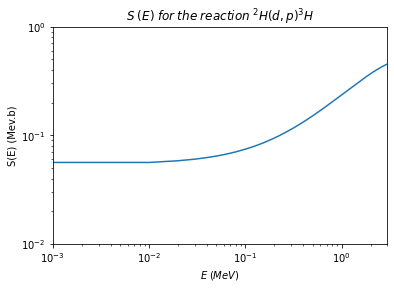
\includegraphics[width=.4\linewidth]{./Figures/S(E) for d(d,p)t.png}}}
    \subfloat[Reaction Rate]{{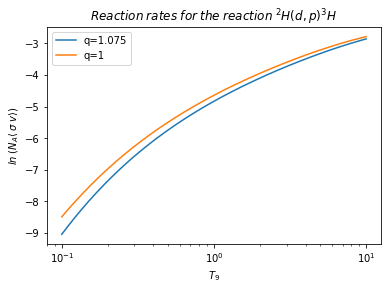
\includegraphics[width=.4\linewidth]{./Figures/reaction rate for d(d,p)t.png}}}
	\caption{S(E) and Reaction Rate for $d(d,p)t$}
	\label{ddpt}
\end{figure}

\begin{figure}[H]
	\centering
	\subfloat[S(E)]{{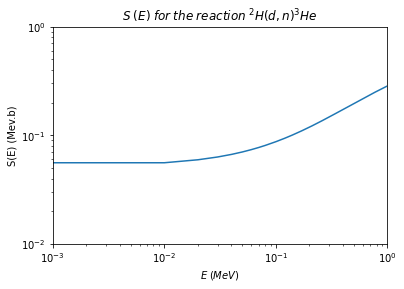
\includegraphics[width=.4\linewidth]{./Figures/S(E) for d(d,n)3He.png}}}
    \subfloat[Reaction Rate]{{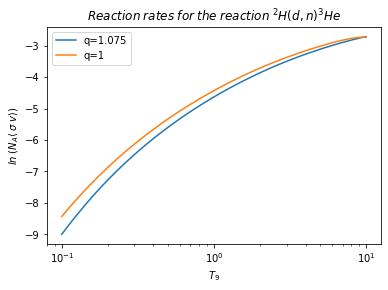
\includegraphics[width=.4\linewidth]{./Figures/reaction rate for d(d,n)3He.png}}}
	\caption{S(E) and Reaction Rate for $d(d,n)^{3}He$}
	\label{ddn3he}
\end{figure}

\begin{figure}[H]
	\centering
	\subfloat[S(E)]{{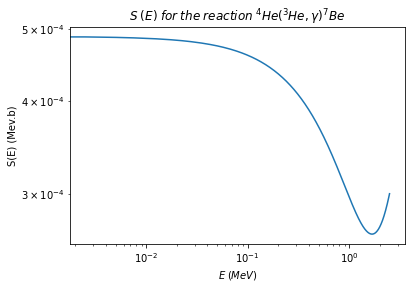
\includegraphics[width=.4\linewidth]{./Figures/S(E) for 4He(3He,gamma)7Be.png}}}
    \subfloat[Reaction Rate]{{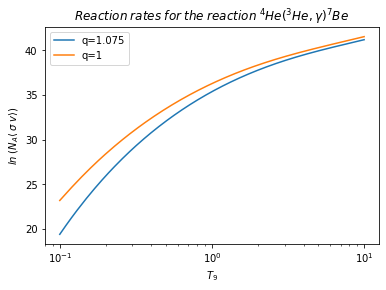
\includegraphics[width=.4\linewidth]{./Figures/reaction rate for 4He(3He,gamma)7Be.png}}}
	\caption{S(E) and Reaction Rate for $^{4}He(^{3}He,\gamma)^{7}Be$}
	\label{4he3heg7be}
\end{figure}

\begin{figure}[H]
	\centering
	\subfloat[S(E)]{{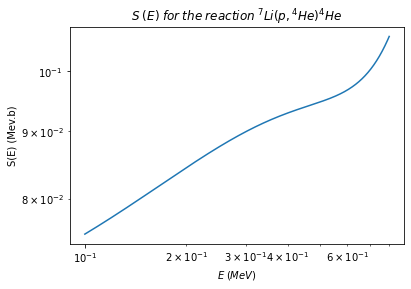
\includegraphics[width=.4\linewidth]{./Figures/S(E) for 7Li(p,4He)4He.png}}}
    \subfloat[Reaction Rate]{{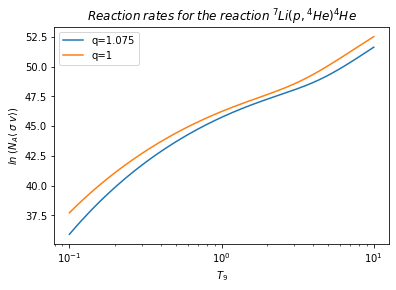
\includegraphics[width=.4\linewidth]{./Figures/reaction rate for 7Li(p,4He)4He.png}}}
	\caption{S(E) and Reaction Rate for $^{7}Li(p,^{4}He)^{4}He$}
	\label{7lip4he4he}
\end{figure}

\begin{figure}[H]
	\centering
	\subfloat[S(E)]{{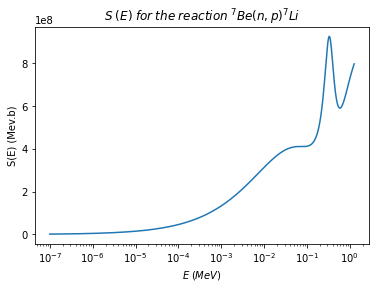
\includegraphics[width=.4\linewidth]{./Figures/S(E) for 7Be(n,p)7Li.png}}}
    \subfloat[Reaction Rate]{{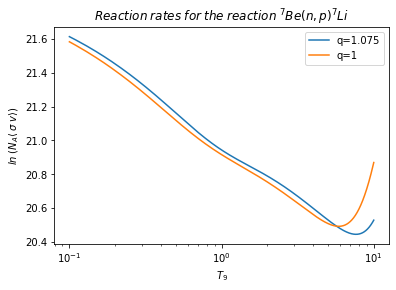
\includegraphics[width=.4\linewidth]{./Figures/reaction rate for 7Be(n,p)7Li.png}}}
	\caption{S(E) and Reaction Rate for $^{7}Be(n,p)^{7}Li$}
	\label{7benp7li}
\end{figure}

\section{Lithium Problem}
\label{sec: Lithium Problem}
The generally accepted prediction for Lithium abundance is the one in \cite{cyburt2016big} that reports $^{7}Li/H = (4.68 \pm 0.67)10^{-10}$, which is about 3 times greater than the widely accepted central value of observations, $^{7}Li/H = (1.58 \pm 0.30)10^{-10}$ (\cite{PITROU20181}).
The figure \ref{fig:Simplified reaction network} shows a simplified network of reactions relevant for BBN and the reactions. The actual full network goes beyond these 12 reactions, but these reactions are the most important for calculating the Lithium abundance.  %The reactions $d(d,p)t$, $d(d,n)^{3}He$, and $d(d,p)t$.\\
The full reaction network involves 30 reactions in total with nuclei of $A\leq 9$. The
thermonuclear forward rates for 11 reactions of primary importance (\cite{smith1993experimental},\cite{Kusakabe:2018dzx}) in the primordial light-element nucleosynthesis have been considered to calculate the abundances. Also, this makes it computationally less expensive. 
\begin{figure}[H]
	\centering
	\subfloat[Reaction Network]{{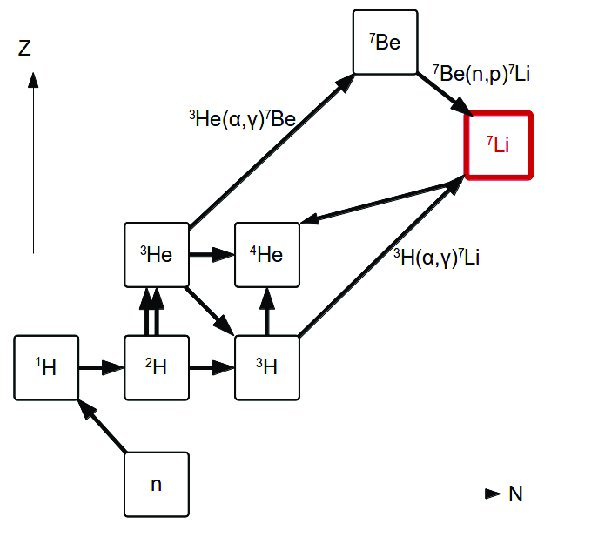
\includegraphics[width=.8\linewidth]{./Figures/Simplified-reaction-network.jpg}}}
    \subfloat[The reactions]{{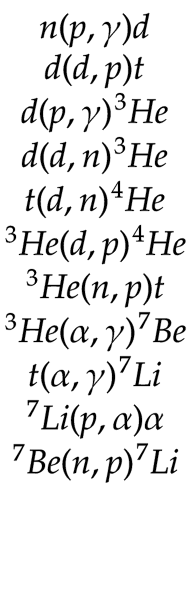
\includegraphics[width=.2\linewidth]{./Figures/math-20220418.png}}}
    \caption{Simplified reaction network showing reactions forming 7 Li during the Big Bang adapted from \cite{Simplified_reaction_network}}
  \label{fig:Simplified reaction network}
\end{figure}

\section{Big Bang Nucleosynthesis code}
The \cite{pypi} package was used to run the Big Bang Nucleosynthesis (BBN) code. The project description is available at: \url{https://pypi.org/project/BBN/#description}, and the files can be found at the author's GitHub page: \url{https://github.com/tt-nakamura/BBN}. The BBN code uses the best fitting curve of the reaction rates as a function of T9 ($10^{9}\; Kelvin$) and the reaction rates are taken from \cite{smith1993experimental}. This code only uses the 12 reactions that that are given in Figure \ref{fig:Simplified reaction network}. \\

\subsection{Getting the best fit Curve for the rate with q-statistics}
Let us consider the reaction $d(d,n)^{3}He$ for demonstrating the procedure. The best fit curve for the reaction rate as given in \cite{smith1993experimental}, is:
\begin{align}
	Rate\;(cm^{3} s^{-1} mole^{-1}) =\; &3.95\times 10^{8} T_{9}^{-2/3}\times \exp(-4.259/T_{9}^{1/3})\times (1.0 + 0.098T_{9}^{1/3} + \nonumber \\
	&0.765T_{9}^{2/3} + 0.525T_{9}+ 9.61\times 10^{-3}T_{9}^{4/3} + 0.0167T_{9}^{5/3})\label{eq:rate fit}
\end{align}
Figure \ref{fig:reaction rate fit} shows the reaction rates for the reaction $d(d,n)^{3}He$. The blue graph corresponds to Equation \ref{eq:rate fit}. The orange and green graphs are the ones from Figure \ref{ddn3he} (The graphs are not in the logarithmic scale in Figure \ref{fig:reaction rate fit})
\begin{figure}[H]
  \centering
  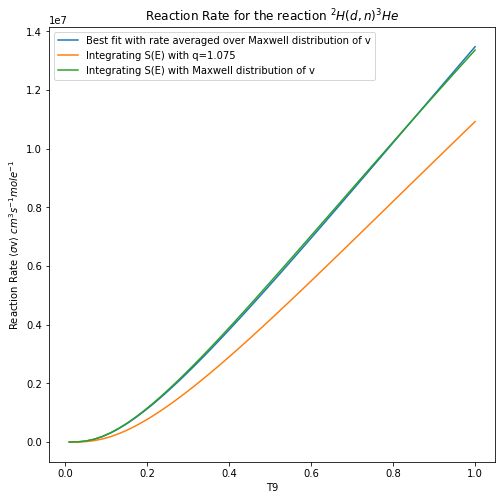
\includegraphics[width=0.7\linewidth]{"./Figures/reaction rate fit.png"}
  \caption{Reaction Rate for $d(d,n)^{3}He$}
  \label{fig:reaction rate fit}
\end{figure}

To find the best fit curve for the graph with q-statistics, we need to find an expression to model the difference between the equation \ref{eq:rate fit} and the q graph. 

\begin{figure}[H]
	\centering
	\subfloat[S(E)]{{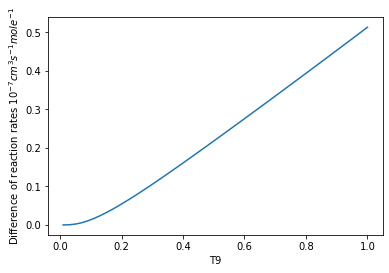
\includegraphics[width=.5\linewidth]{./Figures/difference of reaction rates.png}}}
    \subfloat[Reaction Rate]{{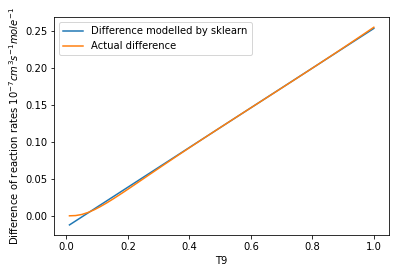
\includegraphics[width=.5\linewidth]{./Figures/model of difference.png}}}
	\caption{Difference of reaction rates and using scikit-learn to get an equation for that difference}
	\label{difference}
\end{figure}

From the library scikit-learn \cite{scikit-learn} which provides tools for data analysis, I have used LinearRegression from sklearn.linear\_model, and PolynomialFeatures from sklearn.preprocessing, to get the best fit curve. Thus, equation \ref{eq:rate fit} becomes:

\begin{align}
	Rate\;(cm^{3} s^{-1} mole^{-1}) =\; &3.95\times 10^{8} T_{9}^{-2/3}\times \exp(-4.259/T_{9}^{1/3})\times (1.0 + 0.098T_{9}^{1/3} + \nonumber \\
	&0.765T_{9}^{2/3} + 0.525T_{9}+ 9.61\times 10^{-3}T_{9}^{4/3} + 0.0167T_{9}^{5/3}) + \nonumber \\
	&(-0.0150250800 + 0.268885978\times T_{9})\times 10^{7} \label{eq:model for rate}
\end{align}

\begin{figure}[H]
  \centering
  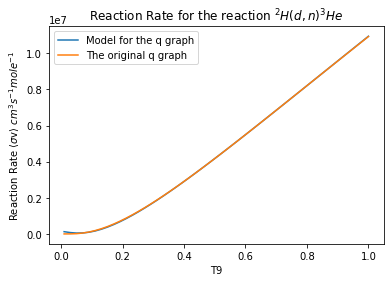
\includegraphics[width=0.7\linewidth]{"./Figures/model of q.png"}
  \caption{Model of the q graph using scikit-learn}
  \label{fig:model of q}
\end{figure}

In the figure \ref{fig:model of q}, the modelled graph coincides with the original q graph. We can use this new reaction rate equation in the BBN code. This method was to all the other important reactions discussed before in \ref{sec: Lithium Problem}

\subsection{Abundance Curves}
\begin{figure}[H]
	\centering
	\subfloat[S(E)]{{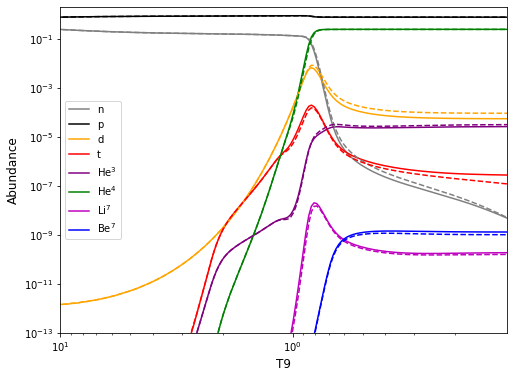
\includegraphics[width=.5\linewidth]{./Figures/abundance temp.png}}}
    \subfloat[Reaction Rate]{{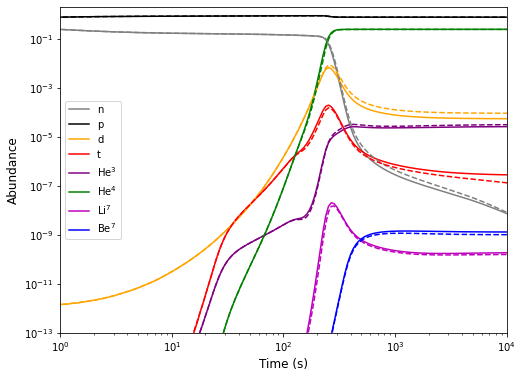
\includegraphics[width=.5\linewidth]{./Figures/abundance time.png}}}
	\caption{Abundance curves as a function of Temperature in figure (a) and Time in figure (b). The solid lines correspond to the MB statistics, and the dotted lines correspond to the Tsallis statistics}
	\label{difference}
\end{figure}

\begin{table}[!ht]
    \centering
    \begin{tabular}{|l|l|l|l|l|}
    \hline
        ~ & MB BBN 
        	& q BBN 
        & Observation 
        & \% Difference \\ \hline
        $^{4} He/H$ & 0.249 & 0.2476 & $0.2561 \pm 0.0108$ & $-3.319\%$ \\ \hline
        $D/H$       & 4.192 & 4.3754 & $3.02\pm 0.23(\times 10^{-5})$ & $38.8\%$ \\ \hline
        $^{3} He/H$ & 0.98 & 1.1793 & $ (1.1 \pm 0.2)(\times 10^{-5})$ & $7.2 \%$ \\ \hline
        $^{7} Li/H$ & 4.39 & 3.7221 & $ (1.58 \pm 0.31)(\times 10^{-10})$ & $15.214 \%$ \\ \hline
    \end{tabular}
\end{table}
The observation values in the above table are taken from \citep{Hou_2017}. From the above table, we can see that this q BBN code follows the trend of \cite{article}. The paper \cite{article} uses the value of q=0.5 and q=2, whereas this code uses the value q=1.075. Due to computational limitations, the code incorporates only the forward reactions. 
We can observe that although the Lithium abundance has decreased, the deuterium abundance has worsened which is consistent with the results in \cite{Kusakabe:2018dzx}. The implications of this are discussed in the next section.

\subsection{Drawbacks of this code}
The reverse reaction rates were not considered due to computational limitations. Although, their affects are more significant at higher temperatures, they still need to be considered for more accurate results.
\\
The Deuterium abundance increases and the $^{7}Li$ abundance decreases with the introduction of the q parameter, which is consistent with \citep{Kusakabe:2018dzx}. This could imply that there is an additional deuterium destruction mechanism. Also, the reduction in the Lithium abundance is still not enough to predict the observed values. But the predictions would be enhanced by adding the reverse reaction rates and considering even more reactions than the ones considered in this project.

\subsection{Future Outlook}
\begin{enumerate}
    \item To calculate the abundances with the reverse reaction rates.

    \item To study the impact of the $\theta$ parameter that was discussed in \autoref{sec: tsallis dist}. Some work on this has been done in \citep{Kusakabe:2018dzx}.

    \item To study the effects of non-extensive statistics in other astrophysics fields as it might offer new perspectives of nucleosynthesis.

\end{enumerate}
\pagebreak

\section{Conclusion}
In this project, the framework of Tsallis non-extensive statistics is used to describe the velocity distribution of nucleons. By adding a non-extensive parameter (q), the abundances of primordial abundances of light nuclei are in better agreement with the observed values. The predictions can be improved by using a more vast code that includes additional reactions along with their reverse reaction rates, where all the rates are calculated in the Tsallis framework. But even with the limitations of this project, we can observe that the Lithium abundances are better predicted in this non extensive framework and this might be a possible solution to the Lithium problem.

 



\pagebreak
\phantomsection

\bibliographystyle{plain}
\bibliography{bibliography}
\addcontentsline{toc}{section}{References}
\end{document}